%====================Step1====================%

%<*mtag100>
\begin{figure}[H]
\centering
\captionsetup{width=1\linewidth}
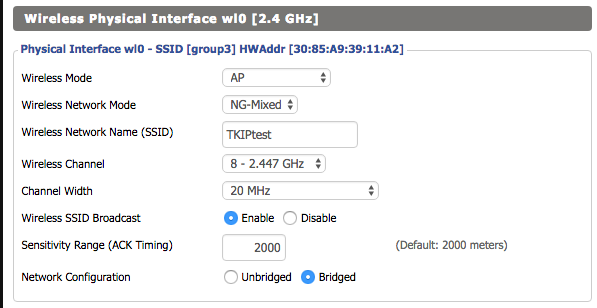
\includegraphics[scale=0.5]{\ImgPath/Ex1/Step1/1.png}
\caption{Shows the configuration of the preliminary TKIP network}
\label{fig:1}
\centering
\end{figure}
%</mtag100>

%<*mtag101>
\begin{figure}[H]
\centering
\captionsetup{width=1\linewidth}
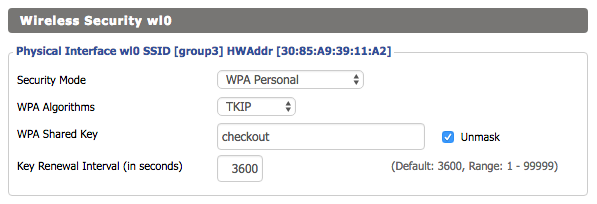
\includegraphics[scale=0.5]{\ImgPath/Ex1/Step1/2.png}
\caption{Changing the security settings of the network}
\label{fig:2}
\centering
\end{figure}
%</mtag101>


%<*mtag102>
\begin{figure}[H]
\centering
\captionsetup{width=1\linewidth}
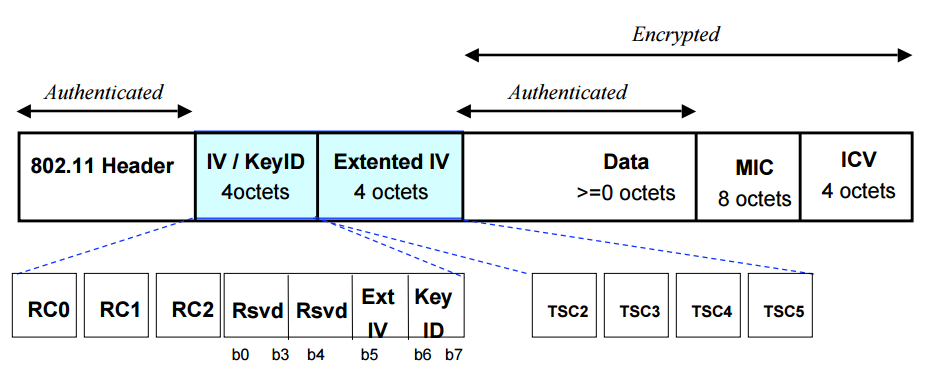
\includegraphics[scale=0.4]{\ImgPath/Ex1/Step1/packet.png}
\caption{Example of the TKIP packet header}
\label{fig:packet}
\centering
\end{figure}
%</mtag102>


%<*mtag103>
\begin{figure}[H]
\centering
\captionsetup{width=1\linewidth}
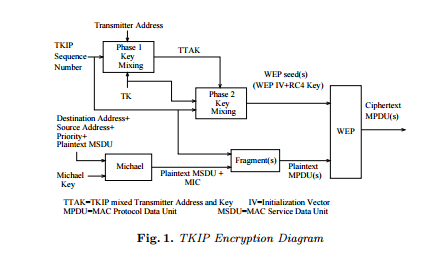
\includegraphics[scale=0.8]{\ImgPath/Ex1/Step1/TKIPflow.png}
\caption{Diagram of the TKIP encryption algorithm and all of its steps.}
\label{fig:TKIPflow}
\centering
\end{figure}
%</mtag103>

%<*mtag104>
\begin{figure}[H]
\centering
\captionsetup{width=1\linewidth}
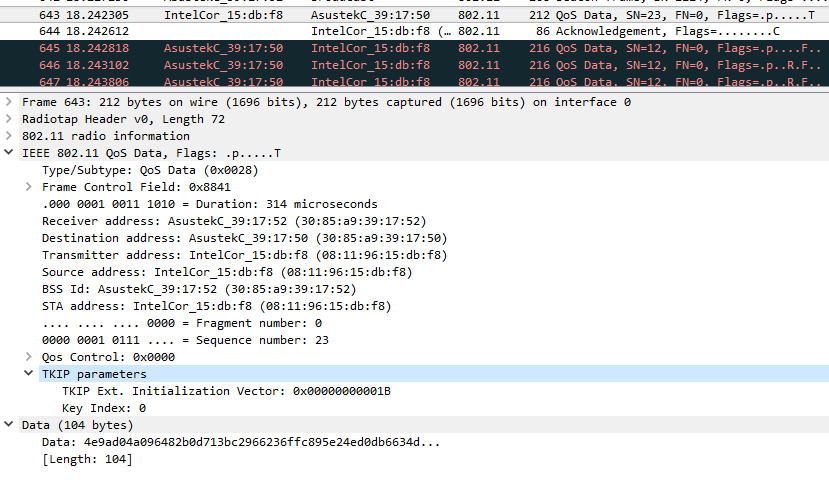
\includegraphics[scale=0.7]{\ImgPath/Ex1/Step1/encrypt.png}
\caption{Example of a encrypted packet in wireshark, with the highlighted TKIP parameters}
\label{fig:encrypt}
\centering
\end{figure}
%</mtag104>

%<*mtag105>
\begin{figure}[H]
\centering
\captionsetup{width=1\linewidth}
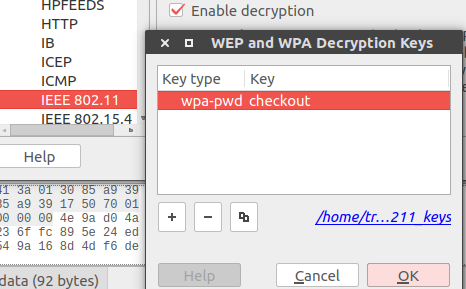
\includegraphics[scale=0.7]{\ImgPath/Ex1/Step1/enableDecrypt.png}
\caption{Going to Edit / Preferences, and entering the Key to decrypt the packet shown in \ref{fig:encrypt}.}
\label{fig:decrypt}
\centering
\end{figure}
%</mtag105>

%<*mtag106>
\begin{figure}[H]
\centering
\captionsetup{width=1\linewidth}
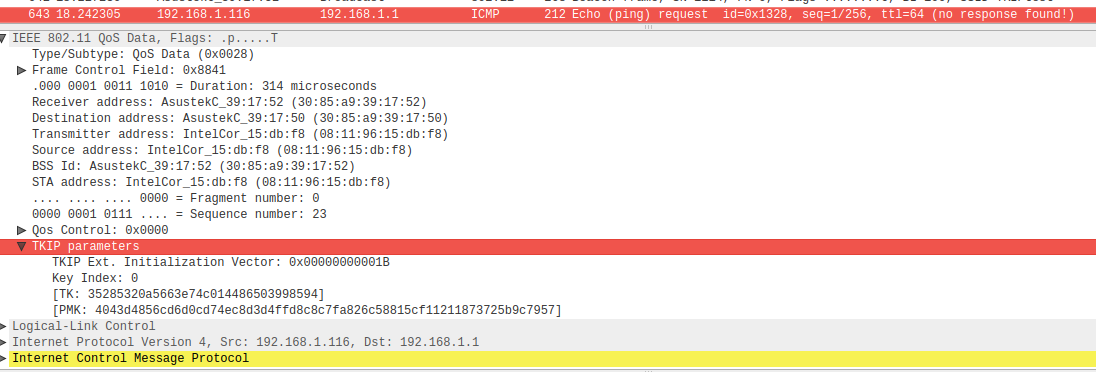
\includegraphics[scale=0.4]{\ImgPath/Ex1/Step1/icmpDecrypt.png}
\caption{Result of decrypting the TKIP packet, with the relevant parameters highlighted}
\label{fig:icmpDecrypt}
\centering
\end{figure}
%</mtag106>

%%STEP 2%%

%<*mtag201>
\begin{figure}[H]
\centering
\captionsetup{width=1\linewidth}
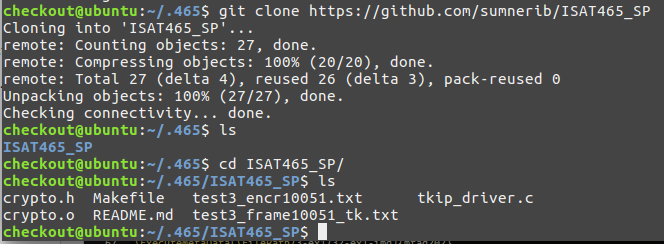
\includegraphics[scale=0.4]{\ImgPath/Ex1/Step2/gitClone.png}
\caption{Cloning the Repository with the relevant C Scripts.}
\label{fig:2-1}
\centering
\end{figure}
%</mtag201>

%<*mtag202>
\begin{figure}[H]
\centering
\captionsetup{width=1\linewidth}
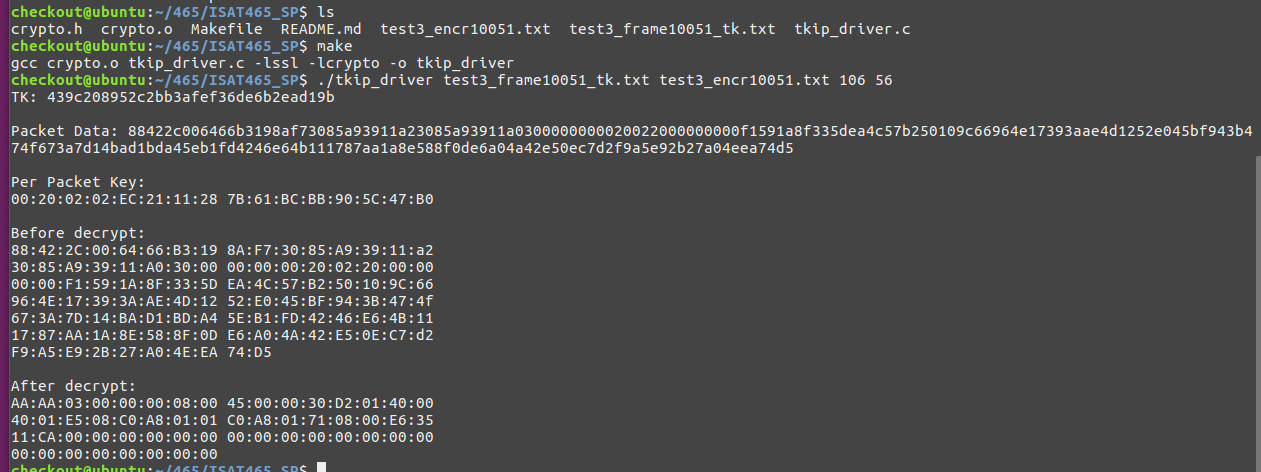
\includegraphics[scale=0.35]{\ImgPath/Ex1/Step2/decryptTKIP.png}
\caption{}
\label{fig:2-2}
\centering
\end{figure}
%</mtag202>

%<*mtag203>
\begin{figure}[H]
\centering
\captionsetup{width=1\linewidth}
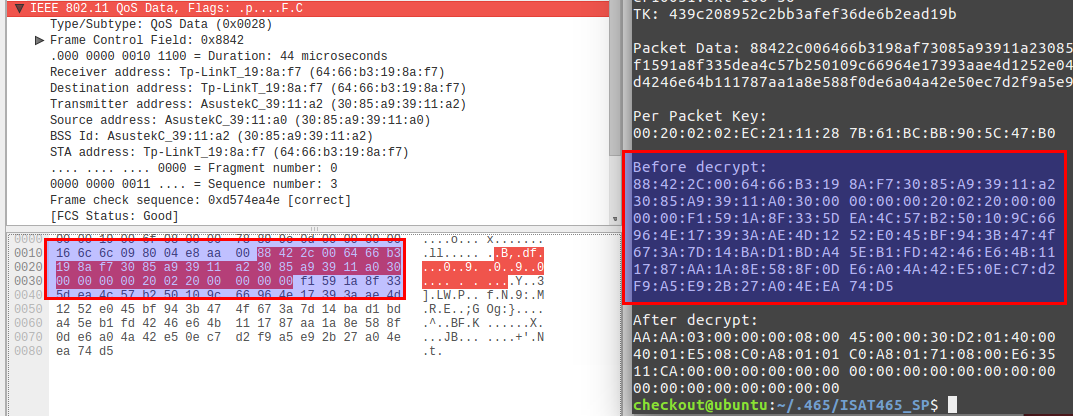
\includegraphics[scale=0.35]{\ImgPath/Ex1/Step2/beforeDecrypt.png}
\caption{Verifying that the data before encryption is consistent with wireshark.}
\label{fig:2-3}
\centering
\end{figure}
%</mtag203>

%<*mtag204>
\begin{figure}[H]
\centering
\captionsetup{width=1\linewidth}
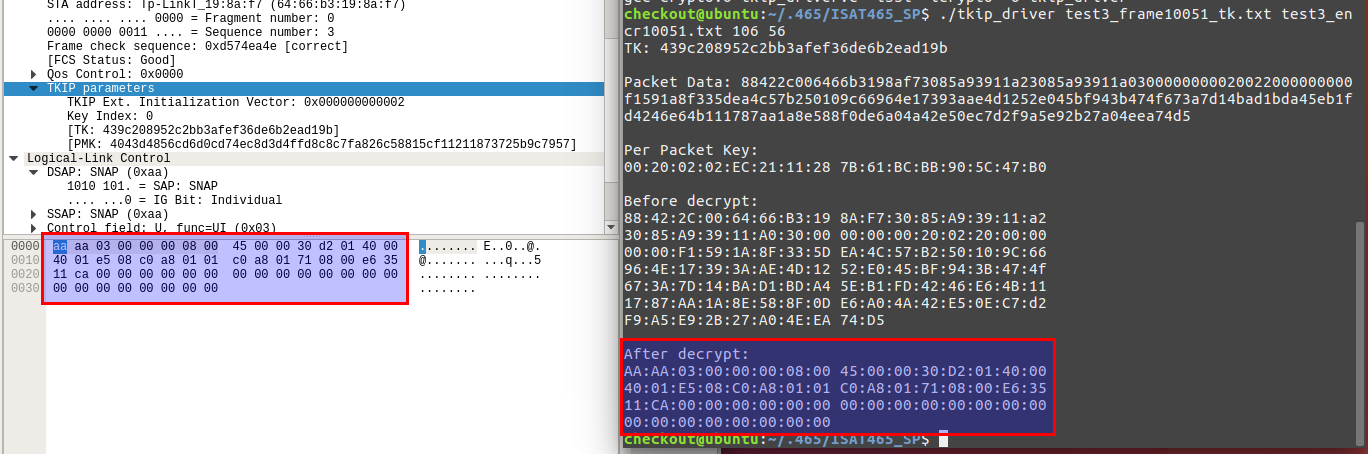
\includegraphics[scale=0.32]{\ImgPath/Ex1/Step2/afterDecrypt.png}
\caption{Confirming that the decryption in the C program is consistent with that of wireshark.}
\label{fig:2-4}
\centering
\end{figure}
%</mtag204>

%<*mtag205>
\begin{figure}[H]
\centering
\captionsetup{width=1\linewidth}
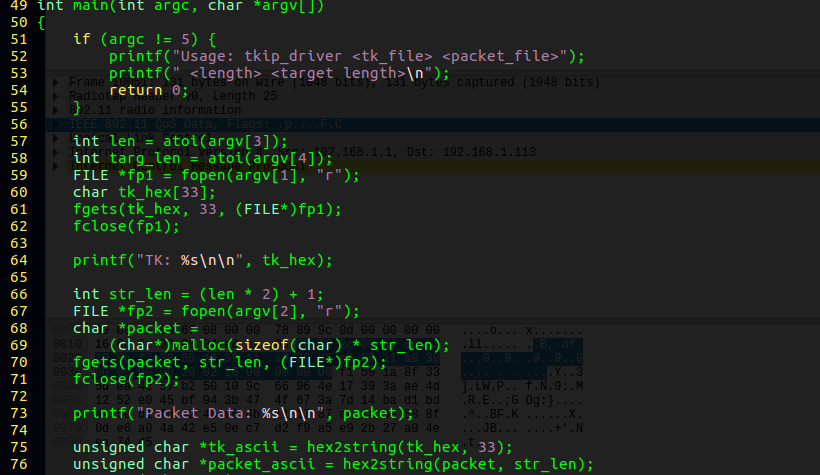
\includegraphics[scale=0.45]{\ImgPath/Ex1/Step2/tkip_driver1.png}
\caption{Beginning of main in the tkip\_driver.c file}
\label{fig:driver1}
\centering
\end{figure}
%</mtag205>

%<*mtag206>
\begin{figure}[H]
\centering
\captionsetup{width=1\linewidth}
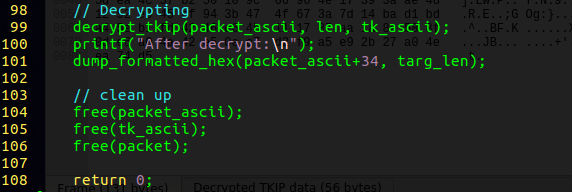
\includegraphics[scale=0.5]{\ImgPath/Ex1/Step2/tkip_driver2.png}
\caption{Calling the decrypt\_tkip function}
\label{fig:driver2}
\centering
\end{figure}
%</mtag206>

%<*mtag207>
\begin{figure}[H]
\centering
\captionsetup{width=1\linewidth}
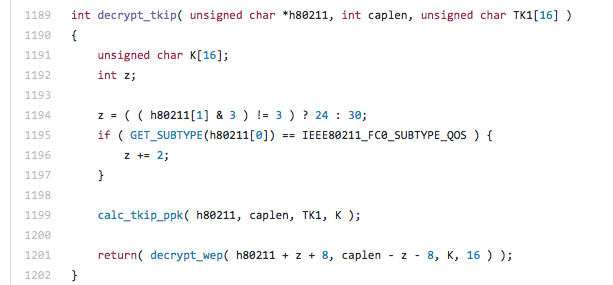
\includegraphics[scale=0.5]{\ImgPath/Ex1/Step2/aircrack1.png}
\caption{The decrypt\_tkip function}
\label{fig:aircrack1}
\centering
\end{figure}
%</mtag207>

%<*mtag208>
\begin{figure}[H]
\centering
\captionsetup{width=1\linewidth}
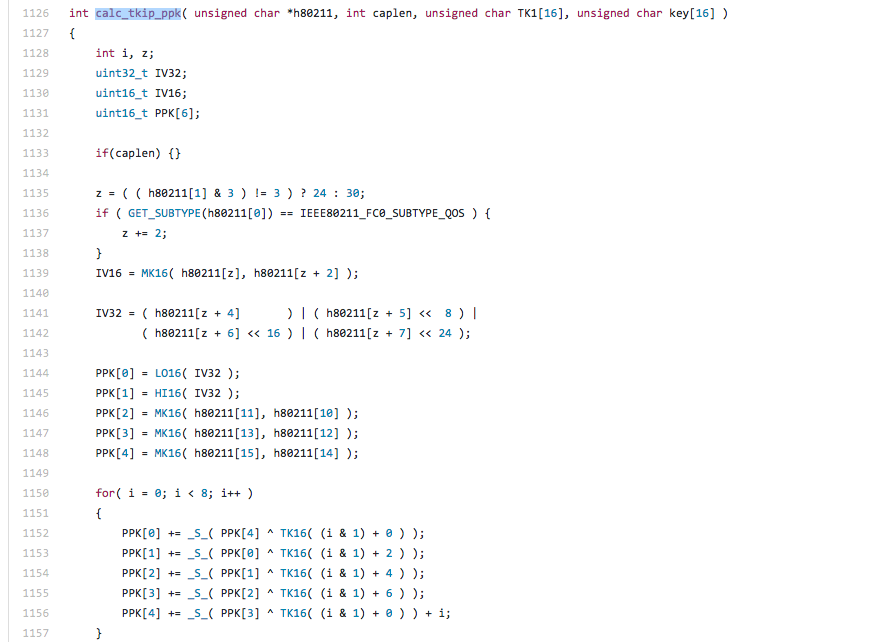
\includegraphics[scale=0.5]{\ImgPath/Ex1/Step2/aircrack2.png}
\caption{Phase 1 of the TKIP Key-mixing Process}
\label{fig:aircrack2}
\centering
\end{figure}
%</mtag208>

%<*mtag209>
\begin{figure}[H]
\centering
\captionsetup{width=1\linewidth}
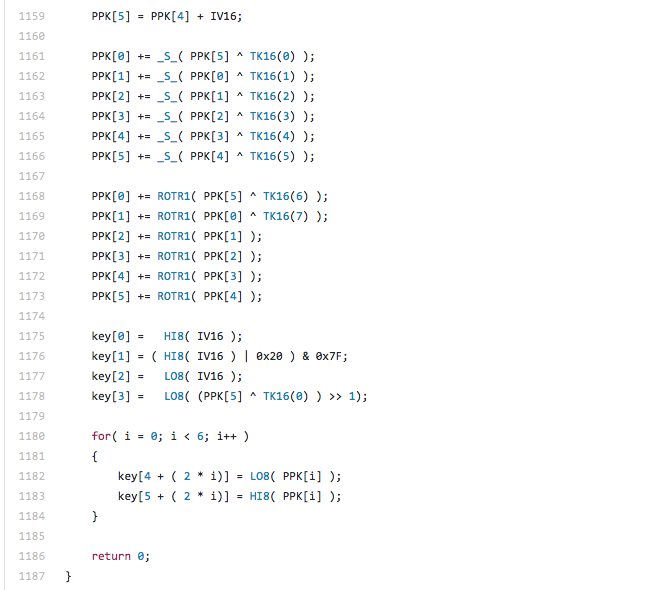
\includegraphics[scale=0.5]{\ImgPath/Ex1/Step2/aircrack3.png}
\caption{Phase 2 of the TKIP Key-mixing Process}
\label{fig:aircrack3}
\centering
\end{figure}
%</mtag209>